\section{Prototypes}
\label{result:prototypes}
Below is a list of features that members of an experience design core team would prefer to have in the tool in question:
\begin{itemize}
  \item List all features of lo-fi prototype here
  \item More lists
\end{itemize}
\subsection{Lo-Fi}
 Several different sketches and concepts were created to obtain a diversity of interfaces to test. Following concepts and elements where selected for the Hi-fi prototyping phase after tests were conducted on all sketches.

\subsubsection{Main interface - Belt UI}
The main interface is designed for the users ergonomic position when seated, displayed from the hip of the user.(Figure \ref{fig:lofi:belt-ui}) The main purpose of this interface is to select new object and place them into the world (Figure \ref{fig:lofi:belt-ui:add}), aswell as to change properties of selected object/objects (Figure \ref{fig:lofi:belt-ui:props}). The centered feature in this UI is the scene-hierarchy, from where objects can be selected and created. The purpose of this approach is to introduce the hierarchy to the user by placing it in direct proximity to the actions that are performed. The users FOV will look like an extension of a work-bench (Figure \ref{fig:lofi:belt-ui:fov})

\begin{figure}
\begin{subfigure}{.5\textwidth}
  \centering
  \includegraphics[width=.8\linewidth]{lo-fi/belt-props.jpg}
  \caption{Properties of a selected object in the belt UI}
  \label{fig:lofi:belt-ui:props}
\end{subfigure}%
\begin{subfigure}{.5\textwidth}
  \centering
  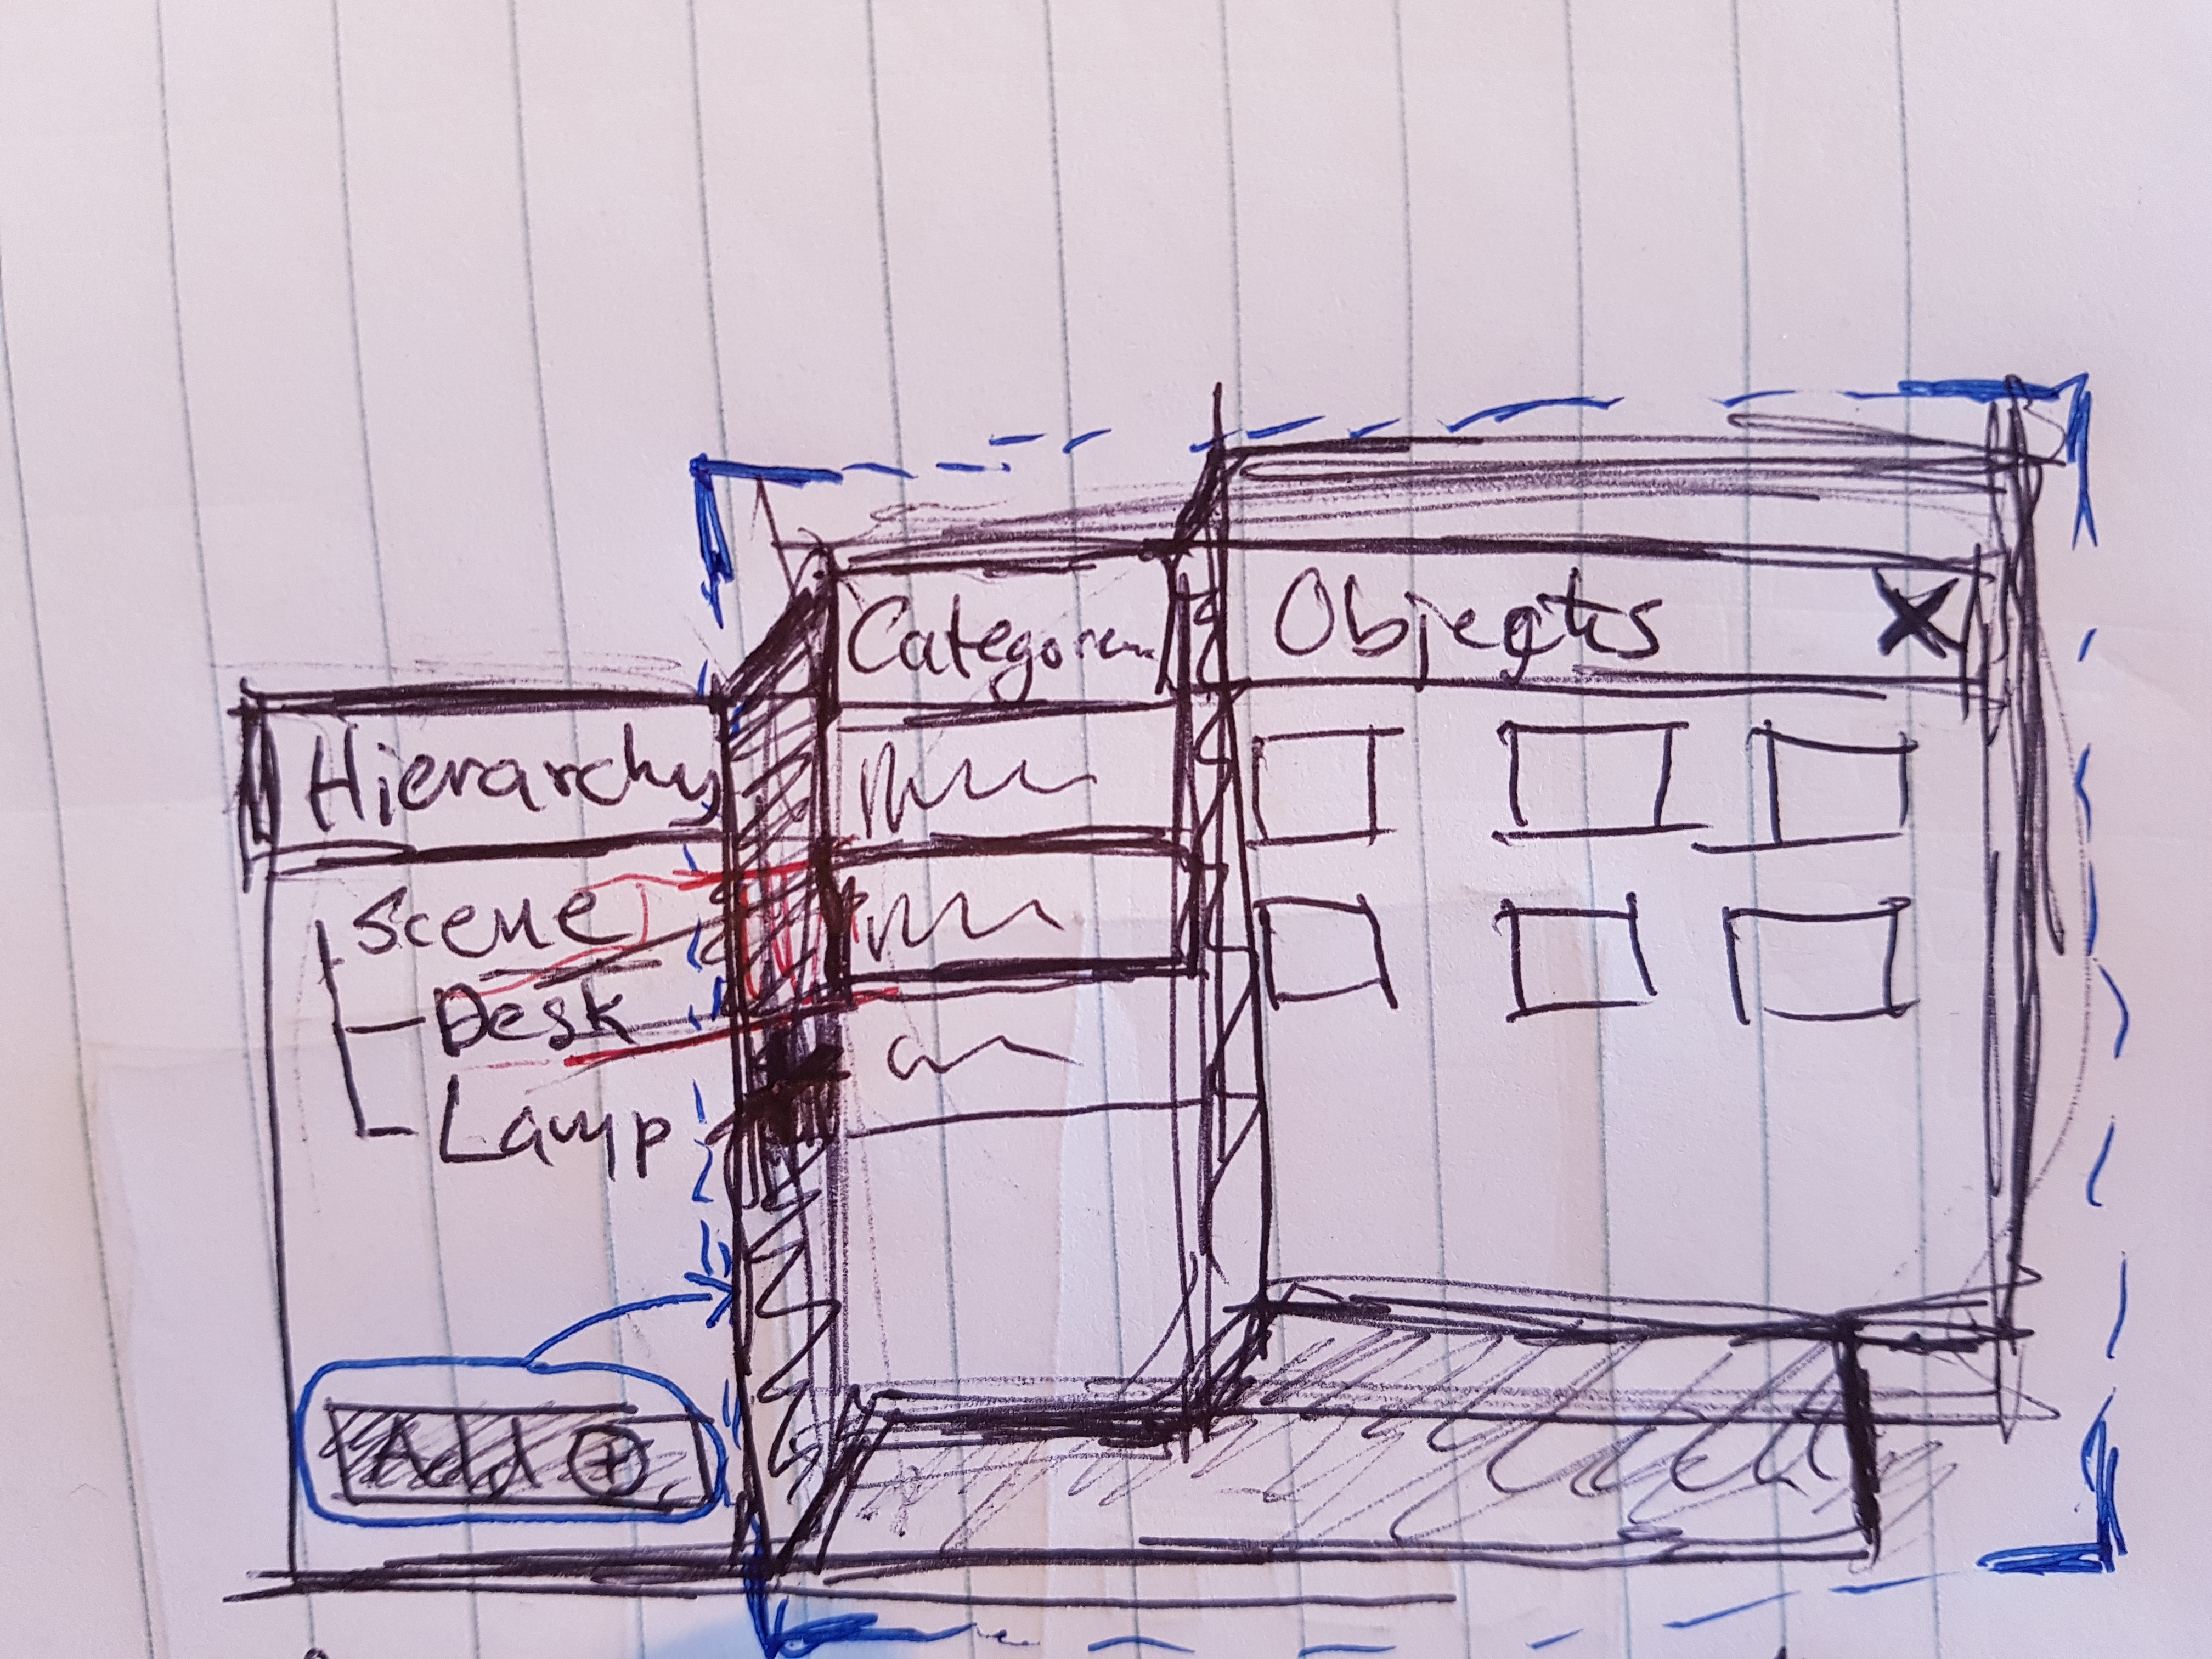
\includegraphics[width=.8\linewidth]{lo-fi/belt-add.jpg}
  \caption{A selection of objects that can be added to the VE}
  \label{fig:lofi:belt-ui:add}
\end{subfigure}
\caption{Paper sketches of the primary UI of the tool: Belt UI}
\label{fig:lofi:belt-ui}
\end{figure}

\begin{figure}
  \begin{subfigure}{.5\textwidth}
  \centering
  \includegraphics[width=.8\linewidth]{lo-fi/belt-perspective.jpg}
  \caption{Field of view for the user with the belt UI open}
  \label{fig:lofi:fov:belt-ui}
  \end{subfigure}%
  \begin{subfigure}{.5\textwidth}
    \centering
    \includegraphics[width=.8\linewidth]{lo-fi/selector-perspective.jpg}
    \caption{Field of view for the user with a visible selector}
    \label{fig:lofi:fov:selector}
\end{subfigure}
\caption{Field of view for the user with different parts of the UI}
\label{fig:lofi:fov}
\end{figure}

\subsubsection{UI Selectors}
A selector is used to manipulate and interact with objects.(Figure \ref{fig:lofi:selector})
\begin{figure}
\begin{subfigure}{.5\textwidth}
  \centering
  \includegraphics[width=.8\linewidth]{lo-fi/selector-submenu.jpg}
  \caption{Accessing a submenu of the selector}
  \label{fig:lofi:selector:select}
\end{subfigure}%
\begin{subfigure}{.5\textwidth}
  \centering
  \includegraphics[width=.8\linewidth]{lo-fi/selector-select.jpg}
  \caption{selection in the selector}
  \label{fig:lofi:selector:submenu}
\end{subfigure}
\caption{multilevel menu selector for objects}
\label{fig:lofi:selector}
\end{figure}


\subsubsection{Object selection and manipulation}
Interaction and techniques for selecting and manipulating objects (Figure \ref{fig:lofi:object}) is explained below

**Missing section: Explaination**

\begin{figure}
\begin{subfigure}{.5\textwidth}
  \centering
  \includegraphics[width=.8\linewidth]{lo-fi/add-object.jpg}
  \caption{Properties of a selected object in the belt UI}
  \label{fig:lofi:object:add}
\end{subfigure}%
\begin{subfigure}{.5\textwidth}
  \centering
  \includegraphics[width=.8\linewidth]{lo-fi/move-object.jpg}
  \caption{A selection of objects that can be added to the VE}
  \label{fig:lofi:object:move}
\end{subfigure}
\caption{Paper sketches of the primary UI of the tool: Belt UI}
\label{fig:lofi:object}
\end{figure}



\subsubsection{Tilt-Brush Tests}
Concepts that appeared to be promising were drawn in Tilt Brush (see Figure \ref{fig:lofi:tilt}) in order to check how perspectives and field of view works in VR.
\begin{figure}
\begin{subfigure}{.5\textwidth}
  \centering
  \includegraphics[width=.8\linewidth]{lo-fi/scalescenario3.PNG}
  \caption{A scale scenario where bottom right corner of a boundingbox is moved}
  \label{fig:lofi:tile:scale3}
\end{subfigure}%
\begin{subfigure}{.5\textwidth}
  \centering
  \includegraphics[width=.8\linewidth]{lo-fi/birdmenu2.PNG}
  \caption{Accessing properties of an object}
  \label{fig:lofi:tilt:passivemenu}
\end{subfigure}
\caption{Lo-fi sketches. Created in Tilt Brush (see Section \ref{relatedwork:tiltbrush})}
\label{fig:lofi:tilt}
\end{figure}
